\documentclass[aspectratio=169]{beamer}
\mode<presentation>
%\usetheme{Warsaw}
%\usetheme{Goettingen}
\usetheme{Hannover}
%\useoutertheme{default}

%\useoutertheme{infolines}
\useoutertheme{sidebar}
\usecolortheme{dolphin}

\usepackage{amsmath}
\usepackage{amssymb}
\usepackage{enumerate}

%some bold math symbosl
\newcommand{\Cov}{\mathrm{Cov}}
\newcommand{\Cor}{\mathrm{Cor}}
\newcommand{\Var}{\mathrm{Var}}
\newcommand{\brho}{\boldsymbol{\rho}}
\newcommand{\bSigma}{\boldsymbol{\Sigma}}
\newcommand{\btheta}{\boldsymbol{\theta}}
\newcommand{\bbeta}{\boldsymbol{\beta}}
\newcommand{\bmu}{\boldsymbol{\mu}}
\newcommand{\bW}{\mathbf{W}}
\newcommand{\one}{\mathbf{1}}
\newcommand{\bH}{\mathbf{H}}
\newcommand{\by}{\mathbf{y}}
\newcommand{\bolde}{\mathbf{e}}
\newcommand{\bx}{\mathbf{x}}

\newcommand{\cpp}[1]{\texttt{#1}}

 \title{Mathematical Biostatistics Boot Camp 2: Lecture 5, Relative Risks and Odds Ratios}
\author{Brian Caffo}
\date{\today}
\institute[Department of Biostatistics]{
  Department of Biostatistics \\
  Johns Hopkins Bloomberg School of Public Health\\
  Johns Hopkins University
}


\begin{document}
\frame{\titlepage}

%\section{Table of contents}
\frame{
  \frametitle{Table of contents}
  \tableofcontents
}

\section{Relative measures}
\begin{frame}\frametitle{Motivation}
  \begin{itemize}
  \item Consider a randomized trial where 40 subjects were randomized (20 each) to 
    two drugs with the same active ingredient but different expedients
  \item Consider counting the number of subjects with side effects for each drug
    \begin{center}
      \ttfamily
      \begin{tabular}{lccc}
        & Side    &      &       \\
        & Effects & None & total \\ \hline
        Drug A & 11           & 9    & 20 \\
        Drug B &  5           & 15   & 20 \\ \hline
        Total  & 16           & 14   & 40 
      \end{tabular}
      \normalfont
    \end{center}
  \end{itemize}
\end{frame}

\begin{frame}\frametitle{Comparing two binomials}
  \begin{itemize}
  \item Let $X \sim \mathrm{Binomial}(n_1, p_1)$ and $\hat p_1 = X / n_1$
  \item Let $Y \sim \mathrm{Binomial}(n_2, p_2)$ and $\hat p_2 = Y / n_2$
  \item We also use the following notation:
    \begin{center}
      \begin{tabular}{|c|c|c|}\hline
        $n_{11} = X$ & $n_{12} = n_1 - X$ & $n_1 = n_{1+}$ \\ \hline
        $n_{21} = Y$ & $n_{22} = n_2 - Y$ & $n_2 = n_{2+}$ \\ \hline
        $n_{+1}$     & $n_{+2}$           &       \\ \hline 
      \end{tabular}
    \end{center}
  \end{itemize}
\end{frame}

\section{The relative risk}
\begin{frame}
  \begin{itemize}
  \item Last time, we considered the absolute change in the proportions, what
    about relative changes?
  \item Relative changes are often of more interest than absolute, eg
    when both proportions are small
  \item The {\bf relative risk} is defined as $p_1 / p_2$
  \item The natural estimator for the relative risk is 
    $$\hat{RR} = \frac{\hat p_1}{\hat p_2} = \frac{X / n_1}{Y / n_2}$$
  \item The standard error for $\log \hat{RR}$  is 
    $$
    \hat{SE}_{\log \hat RR} = \left(\frac{(1 - p_1)}{p_1 n_1} + \frac{(1 - p_2)}{p_2 n_2}\right)^{1/2}
    $$
  \item Exponentiate the resutling interval to get an interval for the
    RR
  \end{itemize}
\end{frame}

\section{The odds ratio}
\begin{frame}
  \begin{itemize}
  \item The {\bf odds ratio} is defined as
    $$
    \frac{\mbox{Odds of SE Drug A}}{\mbox{Odds of SE Drug B}} = 
    \frac{p_1 / (1 - p_1)}{p_2 / (1 - p_2)} = 
    \frac{p_1(1-p_2)}{p_2(1 - p_1)}
    $$
  \item The sample odds ratio simply plugs in the estimates for $p_1$ and $p_2$,
    this works out to have a convenient form
    $$
    \hat{OR} = \frac{\hat p_1 / (1 - \hat p_1)}{\hat p_2 / (1 - \hat p_2)}
    = \frac{n_{11}n_{22}}{n_{12}n_{21}}
    $$
    (cross product ratio)
  \item The standard error for $\log \hat{OR}$ is 
    $$
    \hat{SE}_{\log \hat OR} = \sqrt{\frac{1}{n_{11}} + \frac{1}{n_{12}} +\frac{1}{n_{21}} + \frac{1}{n_{22}}}
    $$
  \item Exponentiate the resulting interval to obtain an interval for
    the OR
  \end{itemize}
\end{frame}

\begin{frame}\frametitle{Some comments}
  \begin{itemize}
  \item Notice that the sample and true odds ratios do not change if we
    transpose the rows and the columns
  \item For both the OR and the RR, taking the logs helps with adherence to the
    error rate
  \item Of course the interval for the log RR or log OR is obtained by taking 
    $$Estimate \pm Z_{1-\alpha/2}SE_{Estimate}$$
  \item Exponentiating yields an interval for the OR or RR
  \item Though logging helps, these intervals still don't perform
    altogether that well
  \end{itemize}
\end{frame}


\begin{frame}\frametitle{Example - RR}
  \begin{itemize}
  \item For the relative risk, $\hat p_A = 11 /20 = .55$, $\hat p_B = 5 / 20 = .25$
  \item $\hat{RR}_{A/B} = .55 / .25 = 2.2$
  \item $\hat{SE}_{\log \hat RR_{A/B}} = \sqrt{\frac{1 - .55}{.55\times20} + \frac{1 - .25}{.25\times 20}} = .44$
  \item Interval for the log RR: ~~$\log(2.2)\pm 1.96 \times .44 = [-.07, 1.65]$
  \item Interval for the RR: ~~ $[.93, 5.21]$
  \end{itemize}
\end{frame}

\begin{frame}\frametitle{Example - OR}
  \begin{itemize}
  \item $\hat{OR}_{A/B} = \frac{11\times 15}{9\times 5} = 3.67$
  \item $\hat{SE}_{\log \hat OR_{A/B}} = \sqrt{\frac{1}{11} + \frac{1}{9} + \frac{1}{5} + \frac{1}{15}} = .68$
  \item Interval for log OR: ~~ $\log(3.67) \pm 1.96 \times .68 = [-.04, 2.64]$
  \item Interval for the OR:  ~~ $[.96, 14.01]$
  \end{itemize}
\end{frame}

\begin{frame}\frametitle{Example - RD}
  \begin{itemize}
  \item For the risk difference $\hat{RD}_{A-B} = \hat p_A - \hat p_B = .55 - .25 = .30$
  \item $\hat{SE}_{\hat  RD_{A-B}} = \sqrt{\frac{.55\times .45}{20} + \frac{.25\times .75}{20}} = .15$
  \item Interval:~~ $.30 \pm 1.96 \times .15 = [.15, .45]$
  \end{itemize}
\end{frame}

\begin{frame}
  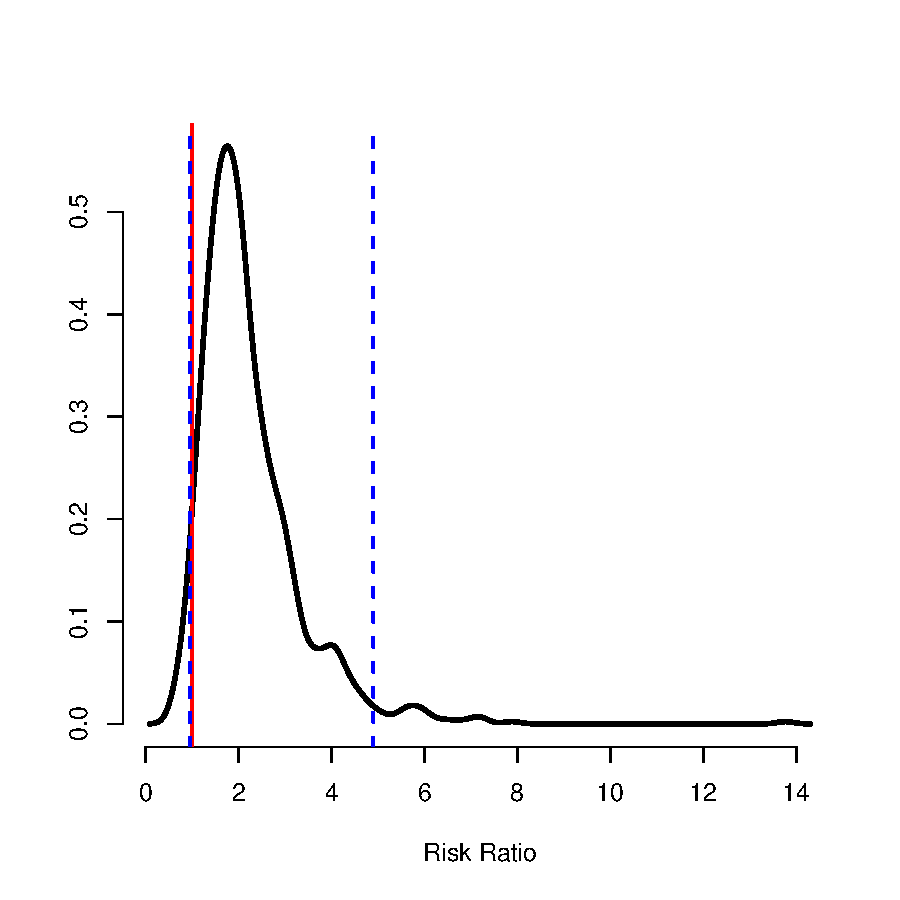
\includegraphics[height=3in]{MCposterior2sampleBinomRR.pdf}
\end{frame}

\begin{frame}
  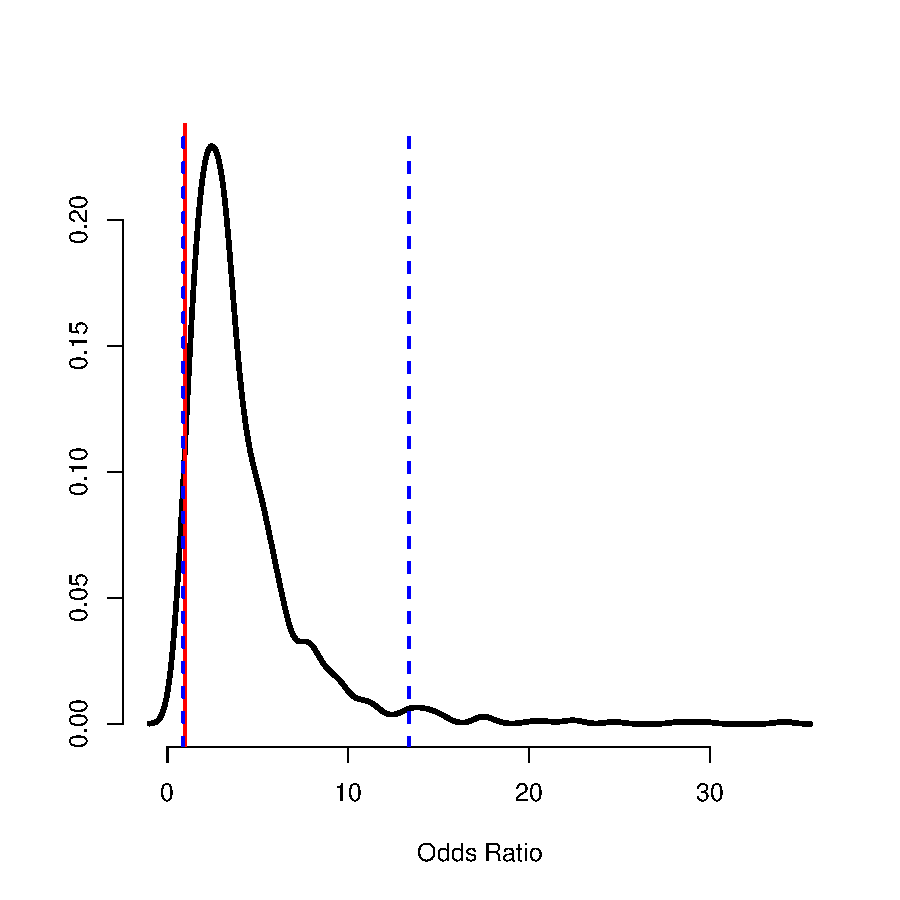
\includegraphics[height=3in]{MCposterior2sampleBinomOR.pdf}
\end{frame}

\end{document}

